%% Class and packages
\documentclass{beamer}
\usepackage[utf8]{inputenc}

%% Metadata
\title{Making data-driven User Recommendations}
\institute{Coursera Capstone}
%\author{meisto}
\date{November 2020}

%% Set theme and colors
\usetheme{Goettingen}
\usecolortheme{default}
\setbeamertemplate{itemize items}[circle]
\setbeamercolor{item projected}{bg=black,fg=white}

%% The actual document
\begin{document}

% Titlepage
\frame{\titlepage}

% Problem
\begin{frame}{What to do at a foreign train station?}
\begin{itemize}
\item Assume your are at a foreign train station, you don't know the city, you don't have personal transport and you have limited time.
\begin{itemize}
\item What can you do?
\item Where can you go?
\item Which places could you like, which not?
\end{itemize}
\item We can use data to make recommendations.
\end{itemize}
\end{frame}

% Data
\begin{frame}{What data do we need?}
\begin{itemize}
\item List of local train stations we can take from our position.
\begin{itemize}
\item Name
\item Location (address, latitude, longitude)
\end{itemize}
\item List of venues near train station.
\begin{itemize}
\item Name
\item Location (address, latitude, longitude)
\item Type (restaurant, bar, \ldots)
\end{itemize}
\end{itemize}
\end{frame}

% Stats 1
\begin{frame}{What can we infer?}
Distribution of different venue types in the city.
\begin{figure}
\centering
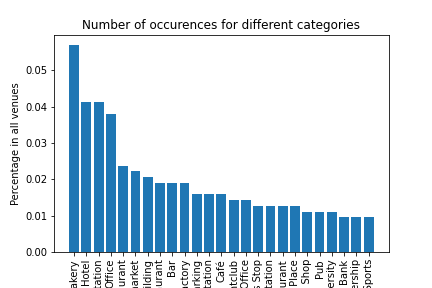
\includegraphics[scale=0.5]{images/dist_overall.png}
\caption{Top 25 venue categories in the dataset.}
\end{figure}
\end{frame}

% Stats 2
\begin{frame}{What do we do with this?}
\begin{itemize}
\item We can group the train stations in groups with a similar venues nearby.
\begin{itemize}
\item Easier to recommend venues.
\item Adjust recommendations to user.
\item Use machine learning.
\end{itemize}
\end{itemize}
\end{frame}

% Stats 3
\begin{frame}{Dividing the city in Clusters}
We can plot these clusters:
\begin{figure}
\centering
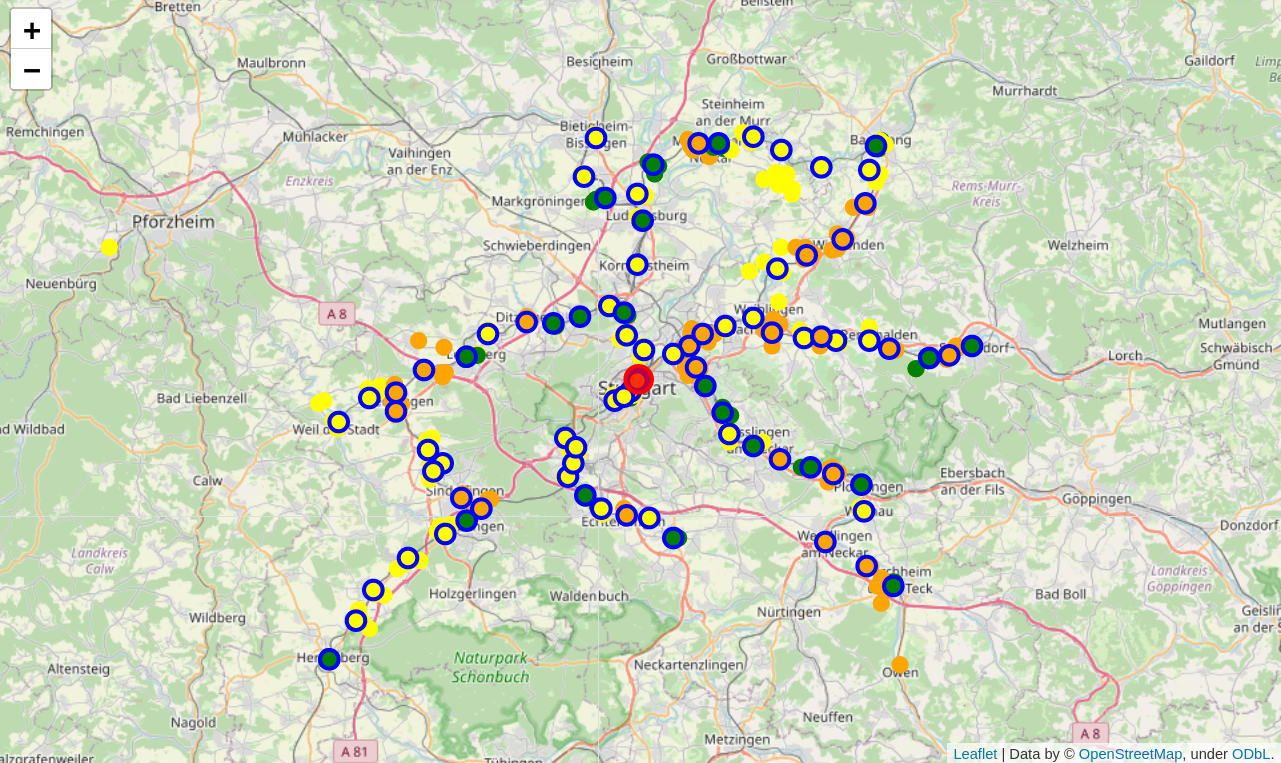
\includegraphics[scale=0.2]{images/spread_cluster.png}
\caption{Plotted stations and venue, color coded by cluster. Unicolor circle are venues, circles with blue borders are station, red circle is exemplary user position.}
\end{figure}
\end{frame}

% Conclusion
\begin{frame}{Conclusion}
\begin{itemize}
\item We saw what data we can use.
\item We saw what inferences we could make.
\item We saw how we can use this data.
\begin{itemize}
\item We can make data-driven recommendation.
\item With a given target wish or just a general recommendation.
\end{itemize}
\end{itemize}
\end{frame}

% Future direction
\begin{frame}{What else can we do?}
\begin{itemize}
\item Add context information for better recommendations.
\item Add other modes of transport.
\item Search in a bigger radius and for more venues.
\item Many possibilities to improve performance even more.
\end{itemize}
\end{frame}

\end{document}
